\documentclass[../main.tex]{subfiles}
\graphicspath{
    {"../img/"}
    {"img/"}
}

\begin{document}
\subsection{Zbiory miary Lebesgue'a zero}

\begin{definicja}
Kostką w $\mathbb{R}^n$ $(a_k \le b_k)$ nazywamy zbiór
\[
    P_k = \left[ a_1,b_1 \right] \times \ldots \times \left[ a_n, b_n \right]
\]
\end{definicja}

\begin{definicja}
    Objętością kostki nazywamy
    \[
        |P_k| = \left\Vert \left[ a_1, b_1 \right]  \right\Vert \cdot \left\Vert \left[ a_2, b_2 \right]  \right\Vert \cdot \ldots\cdot \left\Vert \left[ a_n, b_n \right]  \right\Vert
    ,\]
gdzie $\left\Vert \left[ a_k, b_k \right]  \right\Vert = \left| b_k - a_k \right| $.
\end{definicja}

\begin{definicja}
    Niech $X\in \mathbb{R}^n$. Mówimy, że zbiór $X$ jest miary Lebesgue'a zero, jeżeli
    \[
    \underset{\varepsilon > 0}{\forall}\quad \underset{P = P_1 \cup \ldots \cup P_k}{\exists} : x \subset P, \sum_{i=1}^{k} \left| P_i \right| < \varepsilon
    .\]
\textbf{Uwaga:} $k$ nie musi być wielkością skończoną.
\end{definicja}

\begin{przyklad}
    Niech $\left\{ 1 \right\} \subset \left[ -10, 10 \right] $,
    wówczas
    \[
        \underset{\varepsilon > 0}{\forall} \quad \underset{p = \left[ 1 - \frac{\varepsilon}{4}, 1 + \frac{\varepsilon}{4} \right] }{\exists} : \left\{ 1 \right\} \subset P, \left| P \right|  = \frac{\varepsilon}{2}
    .\]
\end{przyklad}
\begin{przyklad}
    zbiór Cantora\\

\end{przyklad}

    Chcemy dojść do tw Lebesgue.
    \begin{tw}
        (Lebesgue) Niech $P$ - zbiór nieciągłości funkcji $f: D\to\mathbb{R}$, $f$ - ograniczona na $D$, $D$ - \ldots jest zbiorem miary Lebesgue'a zera  $\iff$ $f$ - całkowalna na $D$.
    \end{tw}

    Wiemy, że $f$ - całkowalna $\iff$
    \[
        \underset{\varepsilon>0}{\forall} .\underset{\Pi}{\exists}. |\overline{S}(f,\Pi) - \underline{S}(f,\Pi) | < \varepsilon
    .\]
    \begin{figure}[h]
        \centering
        \includegraphics[width=0.5\textwidth]{fig_33}
    \end{figure}

    Ostatnio pokazaliśmy, że
    \[
        A_{\varepsilon} = \left\{ x\in A, O(f,x) \ge \varepsilon \right\} \text{, to $A_\varepsilon$ jest zbiorem domkniętym}
    .\]
    (PS funkcja $f$ na zbiorze $A$ powinna być ograniczona!!!)
    \begin{figure}[h]
        \centering
        \includegraphics[width=0.5\textwidth]{fig_34}
    \end{figure}

    \begin{obserwacja}
        Jeżeli weźmiemy stól o jakiejś długości to mogę wziąć ileś kartek (albo naleśników. Nie wiadomo czy działa dla czego innego) i go nimi przykryć. Co więcej, jeżeli będzie promocja, to mogę nawet rzucić ich przeliczalnie dużo. Pytanie: czy dla każdego zbioru mogę (niezależnie od kształtu kartek) przykryć go skończoną liczbą kartek?
    \end{obserwacja}

    Weźmy długi stół:
    \begin{align*}
        &R = \bigcup_{n=0}^\infty ] n-2, n+2 [ \cup ]-n-2, -n+2[\\
        &]0,1[ \subset [-2,2]\\
        &]0,1[ \subset [-2019,2018]\cup[-2,2]\\
        &]0,1[ = \bigcup_{n=2}^\infty ]\frac{1}{n},1-\frac{1}{n}[
    .\end{align*}
    Ostatnie jest słabe, bo nie mogę wybrać pokrycia ze skończonej ilości elementów.

    \begin{definicja}
        Niech $X$ - zbiór a $F = \left\{ A_\alpha, \alpha\in\mathbb{R}, A_i, i\in\mathbb{N} \right\} $ - rodzina zbiorów. Mówimy, że $F$ jest pokryciem zbioru $X$, jeżeli $X\subset \bigcup_{i,\alpha}A_\alpha$. Jeżeli zbiory $A_\alpha$ są otwarte, to mówimy, że $F$ jest pokryciem otwartym, jeżeli ilość zbiorów $A_\alpha$ jest skończona, to mówimy, że pokrycie jest skończone. Dowolny podzbiór $F$ taki, że jest też pokryciem zbioru $X$ nazywamy podpokryciem.
    \end{definicja}
    \begin{definicja}
        Zbiór $X$ nazywamy zwartym, jeżeli z \textbf{każdego} pokrycia otwartego możemy wybrać skończone podpokrycie.
    \end{definicja}
    Jak sprawdzamy, czy zbiór jest zwarty, to nie szukamy skończonych pokryć, tylko takie które nie są skończone.
    \begin{stw}
        ($X$ - domknięty,ograniczony) $\iff$ ($X$-zbiór zwarty)
    \end{stw}
    \begin{dowod}
        niech $X\in\mathbb{X}$, $\mathbb{X}$ - przestrzeń metryczna\\
        $\impliedby_1$ Pokażemy, że jeżeli $X$ - zwarty, to $X$ - ograniczony. (przypomnienie: zbiór $A\subset\mathbb{X}$ jest ograniczony jeżeli $\underset{r}{\exists} . \underset{x_0\in A}{\exists} $, że $A\subset K(x_0,r)$
        \begin{figure}[h]
            \centering
            \includegraphics[width=0.5\textwidth]{fig_35}
            \caption{Nieważne, co $A$ myśli o sobie, jeżeli otoczymy je kulą, to jest ograniczone i koniec}
        \end{figure}
        Skoro $X$ - zwarty, to niech $F$ będzie pokryciem złożonym z $K(x,1), x\i X$. $F = \left\{ K(x,1), \underset{x\in X}{\forall}  \right\} $. $F$ jest pokryciem zbioru $X$, ale ponieważ $X$ - zwarty, to znaczy, że z pokrycia $F$ możemy wybrać \textbf{skończone} podpokrycie, co oznacza, że zbiór $X$ możemy ułożyć w kulę o skończonym promieniu. Zatem $X$ - ograniczony.
        \begin{figure}[h]
            \centering
            \includegraphics[width=0.8\textwidth]{fig_36}
            \caption{Przykrywanie zbioru kulami}
        \end{figure}

        $\impliedby_2$ Pokażemy, że $X$ - zwarty, to $X$ - domknięty. Pokażemy, że $X'$ - zbiór otwarty.
        Czyli, że dla dowolnego $p\in X' \underset{K(p,\tilde r)}{\exists} $, że $K(p,\tilde r)\cap X = \phi$ co będzie oznaczało, że $X'$ składa się wyłącznie z punktów wewnętrznych.
        \begin{figure}[h]
            \centering
            \includegraphics[width=0.8\textwidth]{fig_37}
        \end{figure}
    Weźmy $q\in X$, utwórzmy dwa otoczenia:
    \[
        K(q,r), K(p,r); r=\frac{1}{2}d(p,q)
    .\]
    Widać, że $K(q,r) \cap K(p,r) = \phi$. Powtarzamy taką procedurę dla każdego $q\subset X$,
    oznacza to, że dostaniemy pokrycie zbioru $X$ kulami $K(q,r_q), q\in X$, ale $X$ jest zbiorem zwartym więc mogę wybrać \textbf{skończoną} ilość kul \\
    $K(q_1,r_1), K(q_2,r_2),\ldots,K(q_k,r_k)$ będącą pokryciem zbioru $X$.
    \begin{figure}[h]
        \centering
        \includegraphics[width=0.8\textwidth]{fig_38}
    \end{figure}
    A to znaczy, że
    \[
        \underbrace{\left( K(p,r_1)\cap K(p,r_2) \cap \ldots \cap K(p,r_k) \right)}_{\text{jest do zbiór niepusty i \textbf{otwarty}}} \cap \underbrace{\left( K(q_1,r_1) \cup K(q_2,r_2) \cup \ldots \cup K(q_k,r_k) \right)}_{\text{Pokrywa cały $X$}} = \phi
    .\]
    czyli np. \[
        \bigcap_{n=1}^\infty ]-\frac{1}{n}, \frac{1}{n}[ = [0]
    .\]
    Znaleźliśmy otoczenie otwarte punktu $P$ : $K(p,r_k) \cap \ldots K(p,r_k)$, takie, że nie ma punktów wspólnych z $X$, więc $p$ jest punktem wewnętrznym, czyli  $X'$ - otwarty, czyli $X$ - domknięty.

     $X$ - domknięty i ograniczony $\implies$ $X$ - zwarty. Niech $P$ - kostka z $\mathbb{R}^n$, metryka $d_2$. Pokażemy, że $P$ jest zwarta.
    \[
        P = [a_1,b_1]\times\ldots\times[a_n,b_n]
    .\]
    \[
        \lnot(p\implies q)\iff p\land \lnot q
    .\]
    Dowód przez sprzeczność:\\
    Załóżmy, że $P$ - domknięty i ograniczony i $P$ nie jest zwarty. Co to znaczy, że $P$ nie jest zwarte? Oznacza to, że istnieje pokrycie zbioru $P$ takie, że nie da się wyciągnąć z niego skończonego podpokrycia.

    Jeżeli $P$ nie da się pokryć skończoną ilością zbiorów, to znaczy, że jeżeli weźmiemy kostkę $[a_1,c_1]\times[a_2,c_2]\times\ldots\times[a_n,c_n]$ gdzie $c_1 = \frac{a_1+b_1}{2}, c_2 = \frac{a_2+b_2}{2}, \ldots, c_n = \frac{a_n+b_n}{2}$,\\
    to jej też nie możemy podzielić na skończoną ilość elementów. Czyli $P_1\subset P$, kulę $P_1$ też możemy podzielić na cztery części itd\ldots W efekcie dostaniemy ciąg kostek $P P_1 P_2 P_3 \ldots P_n \ldots$.
    Weźmy ciąg elementów
    \begin{align*}
        &x_0\in P\\
        &x_1\in P_1\\
        &\vdots\\
        &x_n\in P_n\\
        &\vdots
    .\end{align*}
    Znaczy, że ciąg $\left\{ x_n \right\}$ jest ciągiem Cauchy (bo każdy element ciągu asdasd). Ciąg $\left\{ x_n \right\} \in\mathbb{R}^n$ czyli $X_n$ jest zbieżny.
    (bo $\mathbb{R}^n$ - zupełna). Niech $\tilde x$ będzie granicą $\left\{ x_n \right\} $ a zbiór $\left\{ P,P_1,P_2,\ldots,P_n,\ldots \right\} $ jest pokryciem $P$ takim, z którego nie możemy wyciągnąć skończonego podpokrycia. Ale skoro $\lim_{n\to\infty}x_n = \tilde x$, to znaczy, że
    \[
        \underset{\varepsilon>0}{\forall} . \underset{n}{\exists} . \underset{n>N}{\forall} . x_n\in K(\tilde x,\varepsilon)
    .\]
    Oznacza to, że mogę tak dobrać $\varepsilon$, że w $K(\tilde x,\varepsilon)$ będą się zawierać wszystkie $P_{i}, i>n$. Mogę wtedy wybrać \textbf{skończone} podpokrycia kostki $P$.\\
    \[
        \left\{ P_1,P_2,P_3,\ldots,P_{n_i}, K(\tilde x,\varepsilon) \right\}
    .\] i sprzeczność
    \begin{figure}[h]
        \centering
        \includegraphics[width=0.5\textwidth]{fig_39}
        \caption{mogę wybrać sobie takie kółko, że wszytkie następne kwadraty będą już leżały w tym kółku!}
    \end{figure}
    \end{dowod}

    Wracamy do tw. Lebesgue'a.
    Obserwacja: Niech $D$ - zwarty, $D\subset \mathbb{R}^n$, $f: D\to \mathbb{R}$ - ograniczona i niech $A = \left\{ x\in D, o(f,x) < \varepsilon \right\} $. Wówczas:
    \[
        \underset{\Pi}{\exists} . |\overline{S}(f,\Pi) - \underline{S}(f,\Pi)|<\varepsilon |D|
    .\]
    \begin{figure}[h]
        \centering
        \includegraphics[width=0.8\textwidth]{fig_40}
    \end{figure}
    \begin{dowod}
        Skoro $\underset{x\in A}{\forall} \lim_{r\to 0} | \underset{K(x',r)}{sup} f(x') - \underset{x'\in K(x',r)}{inf} f(x') | < \varepsilon$
        To znaczy, że
        $\underset{r_\varepsilon}{\exists} $ takie, że $|sup f(x') - inf f(x') | < \varepsilon$.
        Jeżeli zbadamy wszystkie kule $K(x,r_\varepsilon) \underset{x\in D}{\forall} $ to otrzymamy pokrycie $A$. Ale $A$ jest zbiorem zwartym, więc możemy wybrać skończone podpokrycie, czyli skończoną ilość kul takich, że
        \[(*)
            A \subset K(x_1,r_\varepsilon^1)\cup K(x_2,r_\varepsilon^2)\cup\ldots\cup K(x_n,r_\varepsilon^n)
        .\]
        Możemy zatem wybrać podział $\Pi$ zbioru $D$ zgodny z podziałem $(*)$, w wyniku czego,
        \[
            |\overline{S}(f,\Pi) - \underline{S}(f,\Pi)|<\varepsilon |D|
        .\]
    \end{dowod}

\end{document}
